\documentclass[a5paper]{article}
\usepackage[a5paper, top=8mm, bottom=8mm, left=8mm, right=8mm]{geometry}

\usepackage{polyglossia}
\setdefaultlanguage[babelshorthands=true]{russian}

\usepackage{fontspec}
\setmainfont{FreeSerif}
\newfontfamily{\russianfonttt}[Scale=0.7]{DejaVuSansMono}

\usepackage[font=scriptsize]{caption}

\usepackage{amsmath}
\usepackage{amssymb,amsfonts,textcomp}
\usepackage{color}
\usepackage{array}
\usepackage{hhline}
\usepackage{cite}

\usepackage[hang,multiple]{footmisc}
\renewcommand{\footnotelayout}{\raggedright}

\PassOptionsToPackage{hyphens}{url}\usepackage[xetex,linktocpage=true,plainpages=false,pdfpagelabels=false]{hyperref}
\hypersetup{colorlinks=true, linkcolor=blue, citecolor=blue, filecolor=blue, urlcolor=blue, pdftitle=1, pdfauthor=, pdfsubject=, pdfkeywords=}

\usepackage{tabu}

\usepackage{graphicx}
\usepackage{indentfirst}
\usepackage{multirow}
\usepackage{subfig}
\usepackage{footnote}
\usepackage{minted}
\usepackage{xcolor}

\newcommand{\attribution}[1] {
    \vspace{-5mm}\begin{flushright}\begin{scriptsize}\textcolor{gray}{\textcopyright\, #1}\end{scriptsize}\end{flushright}
}

\sloppy
\pagestyle{plain}

\title{Практика 5: Моделирование поведения}
\author{Юрий Литвинов\\\small{yurii.litvinov@gmail.com}}

\date{14.03.2022}

\begin{document}

\maketitle
\thispagestyle{empty}

\section{Диаграммы последовательностей}

На этом занятии предлагается порисовать несколько менее часто встречающиеся диаграммы, использующиеся в основном для моделирования поведения разрабатываемых систем. Первая из них --- это диаграмма последовательностей (sequence diagram). Такие диаграммы очень полезны при анализе асинхронных и параллельных программ, вот напоминание их синтаксиса:

\begin{center}
    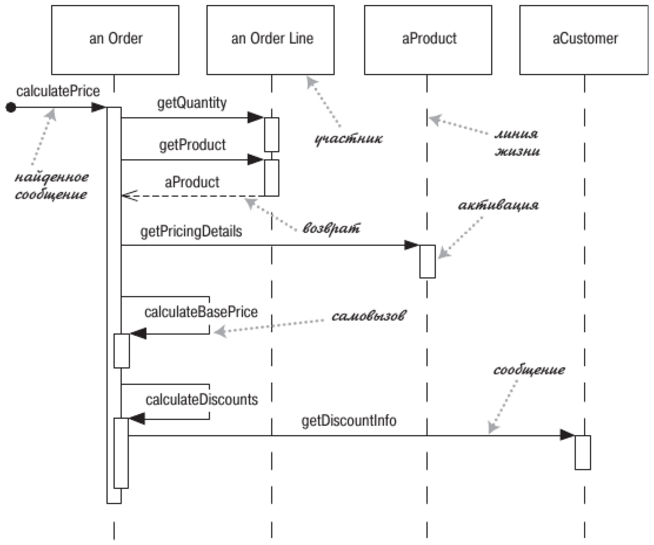
\includegraphics[width=0.8\textwidth]{sequenceDiagram.png}
    \attribution{М. Фаулер, UML. Основы}
\end{center}

На что стоит обратить внимание при рисовании диаграмм на практике:

\begin{itemize}
    \item сообщение может быть послано только активным объектом, поэтому не может выходить из просто линии жизни, нужно линию активации;
    \item сообщение надо обработать, поэтому его получение порождает линию активации хотя бы ненадолго;
    \item объект не может проснуться сам собой, так что линия активации может начаться только с приёма сообщения;
    \item если вы хотите смоделировать асинхронную систему, где непонятно, когда придёт то или иное сообщение, рисуйте его источник как актора --- у него линия жизни вся покрыта активацией; или не рисуйте вовсе, есть <<найденное сообщение>>, оно не требует источника;
    \item возврат имеет смысл рисовать, только если нам важно, что или когда вернули, в остальных случаях возврат просто подразумевается.
\end{itemize}

Можно показывать явное создание и удаление объектов:

\begin{center}
    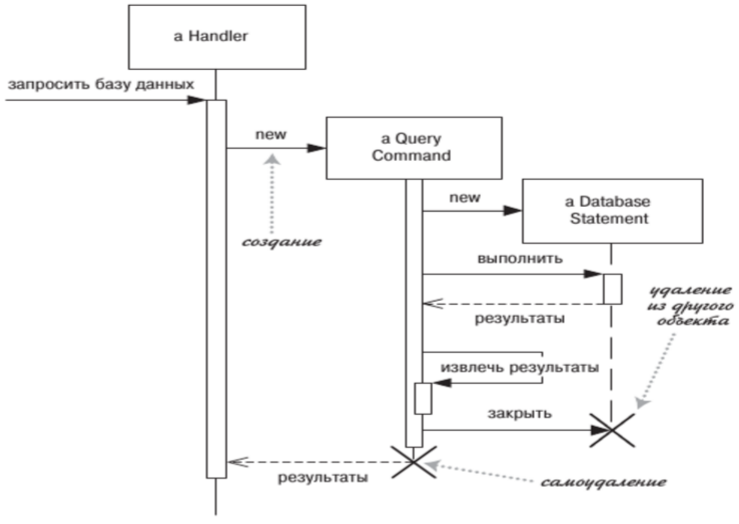
\includegraphics[width=0.7\textwidth]{sequenceLifeCycle.png}
    \attribution{М. Фаулер, UML. Основы}
\end{center}

А можно описать последовательность сообщений в зависимости от каких-то условий, циклы и даже полноценный алгоритм, с помощью фреймов:

\begin{center}
    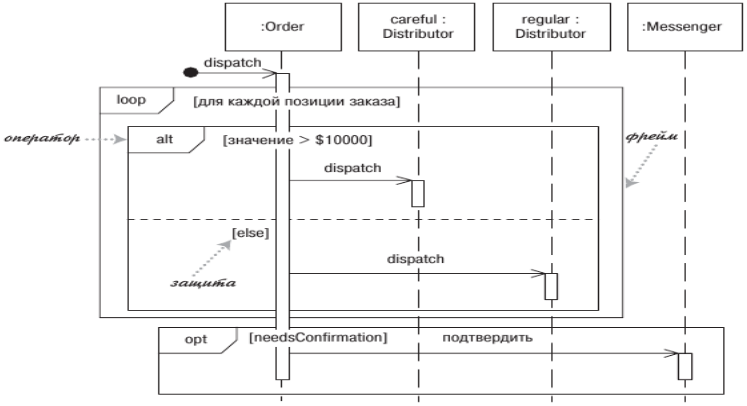
\includegraphics[width=0.6\textwidth]{sequenceFrames.png}
    \attribution{М. Фаулер, UML. Основы}
\end{center}

Вообще фреймы сильно ухудшают читабельность диаграммы, а для визуализации алгоритмов есть средства получше --- диаграммы активностей, например. Так что фреймы --- очень ситуационная штука.

\section{Диаграммы конечных автоматов}

Диаграммы конечных автоматов (также известные как диаграммы состояний) --- это на самом деле несколько упрощённые диаграммы Харела, предложенные им ещё в 1987 году, которые попали в UML с минимальными изменениями. Они использовались и задолго до Харела, конечно, однако у Харела (и в UML) они хитрее, чем обычно ожидают от конечных автоматов, в частности, поддерживают вложенные и параллельные состояния.

Напоминание о синтаксисе:

\begin{center}
    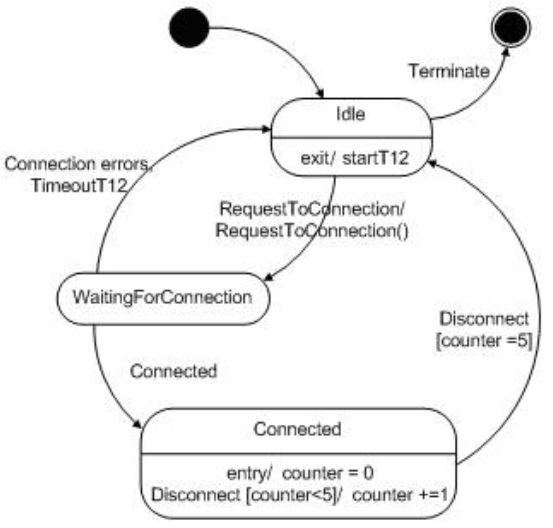
\includegraphics[width=0.4\textwidth]{stateTransitionExample.png}
\end{center}

Внешне диаграммы конечных автоматов похожи на диаграммы активностей, поэтому их часто путают и из-за этого рисуют неправильно (в этом есть смысл, в UML до версии 2 эти диаграммы не разделялись). Есть важные семантические различия:

\begin{itemize}
    \item на диаграмме активностей рисуются активности, система в них не задерживается, а сразу переходит дальше; на диаграмме конечных автоматов рисуются состояния --- стабильные отрезки жизненного цикла объекта, в которых он находится большую часть времени и может из них выйти только если что-то произойдёт;
    \item полезная работа на диаграммах активностей производится в активностях, на диаграммах автоматов --- как правило, при переходе;
    \item диаграммы активностей моделируют один метод объекта (или какую-то функцию или что-то такое), диаграммы конечных автоматов --- целый объект (состояния моделируются полями объекта).
\end{itemize}

Более подробно про синтаксис:

\begin{center}
    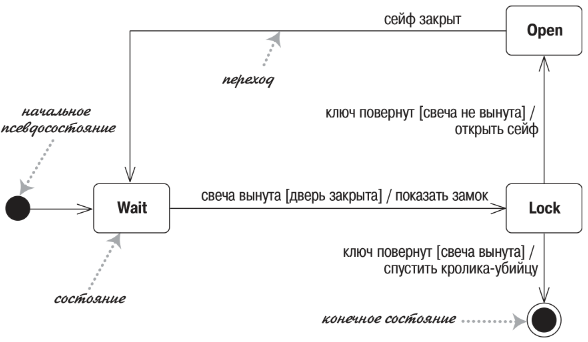
\includegraphics[width=0.7\textwidth]{stateTransitionSyntax.png}
    \attribution{М. Фаулер, UML. Основы}
\end{center}

Внутри состояния могут быть:

\begin{itemize}
    \item entry activity --- то, что делается при входе в состояние по любому из переходов;
    \item exit activity --- то, что делается при выходе из состояния по любому исходящему переходу (и входная, и выходная деятельность --- это, как правило, вызовы метода);
    \item do activity --- деятельность, выполняющаяся всегда, когда система находится в таком-то состоянии (например, попытки подключения к сети для мобильного телефона);
    \item внутренний переход --- переход по событию, который ведёт в то же состояние и не приводит к срабатыванию entry и exit activity. Переход вполне может быть полноценным переходом в то же состояние (рисуется как петля в графе), тогда entry и exit activity работают как обычно, хоть состояние и не меняется.
\end{itemize}

Событие, кстати, это нечто внешнее по отношению к системе, на что система может реагировать. Примеры событий --- действие пользователя, сетевой пакет, считывание символа (если речь идёт об автоматном лексическом анализаторе, который, кстати, хоть и несколько необычный, но тоже пример реактивной системы, которая прекрасно моделируется конечными автоматами).

Надпись на переходе имеет следующий синтаксис: \verb|[<trigger> [‘,’ <trigger>]* [‘[‘ <guard>’]’] [‘/’ <behavior-expression>]]| --- один переход может реагировать на несколько событий сразу, иметь опционального стражника (в квадратных скобках) и через слеш действие (вызов метода или отсылку к диаграмме активностей, которая поясняет, что нужно делать при переходе).

\section{Временные диаграммы}

Временные диаграммы создавались прежде всего для инженеров-электронщиков или для людей, проектирующих системы реального времени, в реальной практике не встречались автору ни разу. Есть два варианта синтаксиса:

\begin{center}
    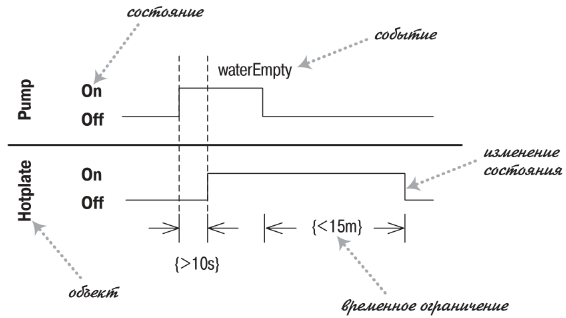
\includegraphics[width=0.6\textwidth]{timingDiagrams.png}
    \attribution{М. Фаулер, UML. Основы}
\end{center}

и

\begin{center}
    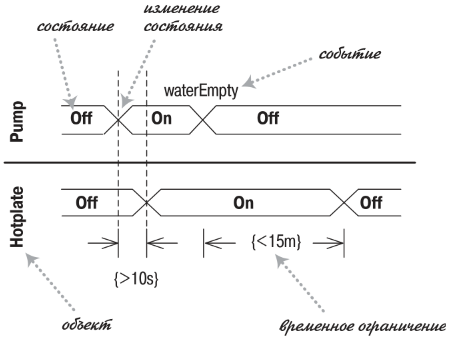
\includegraphics[width=0.6\textwidth]{timingDiagramsAlternate.png}
    \attribution{М. Фаулер, UML. Основы}
\end{center}

В обоих случаях рисуется временная шкала (время идёт слева направо), на ней вертикально располагаются объекты, которые могут находиться в некоторых состояниях. Первый вариант показывает переключение состояния как скачок линии, второй --- как пересечение линий с именем состояния внутри. Второй вариант удобнее, если состояний много, первый вариант нагляднее. Помимо состояний указываются и временные ограничения, в фигурных скобках, как принято в UML для ограничений.

Тонкость в том, что это один из немногих примеров \emph{неграфовых} визуальных языков, поэтому многие редакторы их попросту не умеют. Умеет Visual Paradigm и вроде умеет Creately.

\section{Задание на пару}

Нарисовать следующие диаграммы:

\begin{enumerate}
    \item диаграмму последовательностей регистрации и ремонта дефекта из уже знакомого вам запроса \url{https://bit.ly/defects-rfp};
    \item диаграмму конечных автоматов, описывающую поведение микроволновки;
    \item временную диаграмму любого сценария работы микроволновки;
    \begin{itemize}
        \item в VP это может быть не совсем тривиально: \url{https://www.visual-paradigm.com/support/documents/vpuserguide/94/2586/6715_drawingtimin.html}
        \item в diagrams.net не факт, что вообще возможно, из браузерных решений, наверное \url{https://creately.com/lp/timing-diagram-software/}
    \end{itemize}
\end{enumerate}

\end{document}